% Created 2019-05-15 Wed 23:29
% Intended LaTeX compiler: pdflatex
\documentclass[11pt]{article}
\usepackage[utf8]{inputenc}
\usepackage[T1]{fontenc}
\usepackage{graphicx}
\usepackage{grffile}
\usepackage{longtable}
\usepackage{wrapfig}
\usepackage{rotating}
\usepackage[normalem]{ulem}
\usepackage{amsmath}
\usepackage{textcomp}
\usepackage{amssymb}
\usepackage{capt-of}
\usepackage{hyperref}
\author{Rodda John}
\date{\today}
\title{}
\hypersetup{
 pdfauthor={Rodda John},
 pdftitle={},
 pdfkeywords={},
 pdfsubject={},
 pdfcreator={Emacs 25.2.1 (Org mode N/A)}, 
 pdflang={English}}
\begin{document}



\section{Goals}
\label{sec:org3d5957a}
\begin{itemize}
\item Basic introduction to Computer Science
\item Basic introduction to Python
\item Reading documentation and using Google
\item Simple data analysis in Python
\end{itemize}


\section{What is Computer Science?}
\label{sec:org0e95733}
\begin{itemize}
\item When I say Computer Science, what do you think of?
\item Is it a discipline or a tool?
\item Do you need a computer to study it?
\end{itemize}

\subsection{Formal Definition}
\label{sec:orge852e01}
\begin{quote}
Computer science is the study of the theory, experimentation, and engineering that form the basis for the design and use of computers. It is the scientific and practical approach to computation and its applications and the systematic study of the feasibility, structure, expression, and mechanization of the methodical procedures that underlie the acquisition, representation, processing, storage, communication of, and access to, information.
\end{quote}

\subsection{So\ldots{}}
\label{sec:org8a513fc}
\begin{itemize}
\item Is it a discipline or a tool?
\item Do you need a computer to study it?
\item Disclaimer
\end{itemize}

\section{Let's Begin}
\label{sec:org9ec2b37}
\begin{enumerate}
\item Open IDLE and create a new file
\item Save it as something memorable

\item Type:
\begin{verbatim}
print('Hello World!')
\end{verbatim}
\item Run it
\item Be greeted!
\end{enumerate}

\subsection{But wait, what'd that do}
\label{sec:orgcf3f763}
\begin{itemize}
\item From before:
\begin{verbatim}
print('Hello World!')
\end{verbatim}
\item \texttt{print()} is a function
\item \texttt{'Hello World!'} is an argument
\item So, to generalize:
\begin{itemize}
\item \texttt{print(arg)} prints the \texttt{arg}
\end{itemize}
\end{itemize}
\section{Variables}
\label{sec:orgfe19b2e}
\begin{itemize}
\item Does \texttt{print(Hello world!)} work?
\item Predict first
\item Test it
\item Analyze the error
\begin{itemize}
\item What's the error?
\end{itemize}
\end{itemize}
\subsection{Strings}
\label{sec:orgac1de59}
\begin{itemize}
\item A string is any expression of characters enclosed in \texttt{'} or \texttt{"}
\item Is \texttt{'h'} a string?
\item How about \texttt{h}?
\item What about \texttt{'3'}?
\item How about \texttt{3}?
\item How about \texttt{'Hi, what's up Bob?'}?
\item What about \texttt{"Hi, what's up Bob?"}?
\item So what variable type does the print function accept?
\end{itemize}
\subsection{Numbers}
\label{sec:orgac538f5}
\begin{itemize}
\item A number is a representation of, well, a number\ldots{}
\item \texttt{3} is a number, \texttt{'3'} is not
\item You can do math on numbers!
\item \texttt{3 + 3} is valid Python
\item So is \texttt{3 - 3}, \texttt{3 * 3}, \texttt{3 / 3}, and even \texttt{3 ** 3}.
\item What is \texttt{**}
\item Technically speaking, these are function shortcuts
\begin{itemize}
\item \texttt{3 + 3} is really \texttt{add(3, 3)}
\end{itemize}
\item Try some stuff out
\item Does Python understand parentheses?
\end{itemize}
\subsection{Ok, but what is a variable?}
\label{sec:orge21087e}
It's kinda like a big box

\begin{itemize}
\item Let's see it in action:
\begin{verbatim}
x = 1
y = 2

z = x + y
print(z)

print(x + y)
\end{verbatim}

\item Let's go through our process again:
\begin{itemize}
\item Predict
\item Test
\item Analyze
\end{itemize}
\end{itemize}
\subsection{Same drill}
\label{sec:org5baa393}
Predict, test, analyze\ldots{}

\begin{itemize}
\item Here's another one for you
\begin{verbatim}
x = 'this'
y = 'is'
z = 'a word'

nstring = x + y + z
print(nstring)
\end{verbatim}

\item Given above:
\begin{verbatim}
print(x + y + z)
\end{verbatim}

\item And finally:
\begin{verbatim}
print(x + ' ' + y + ' ' + z)
\end{verbatim}
\end{itemize}

\section{Boolean Expressions}
\label{sec:org399535b}
Just another variable type\ldots{}

\begin{itemize}
\item Can only be \texttt{True} or \texttt{False}
\item What operators could we use to get boolean values?
\item How about to combine two boolean values to one?
\item Let's check this out:
\begin{verbatim}
a, b = 1, 2

x, y = True, False

print(a < b)
\end{verbatim}
\item How about:
\begin{verbatim}
print(x and y)
print(x or y)
print (x and not y)
\end{verbatim}
\end{itemize}
\subsection{Boolean Operators}
\label{sec:orgb7746d2}
Non-Boolean Variables --> Boolean Variables:
\begin{itemize}
\item \begin{center}
\begin{tabular}{ll}
Operator & Description\\
\hline
< & Less than\\
> & Greater than\\
== & Equality\\
<= & lte\\
>= & gte\\
!= & Not equals\\
\end{tabular}
\end{center}
\end{itemize}

\subsection{Boolean Operators}
\label{sec:orge2fee6b}
Boolean Variables --> Boolean Variables:
\begin{itemize}
\item \begin{center}
\begin{tabular}{ll}
Operator & Description\\
\hline
and & logical and\\
or & logical or\\
not & logical not\\
\end{tabular}
\end{center}
\end{itemize}
\subsection{Um, why can't we just use \texttt{=} for equality}
\label{sec:orga2210ff}
Like normal people\ldots{}
\begin{itemize}
\item Do we already have \texttt{=} in python?
\item What does it do?
\item Consider:
\begin{verbatim}
x = 1

x == 1
\end{verbatim}
\item Do we want them to be interchangeable?
\end{itemize}

\section{Control Structures}
\label{sec:org9d6b3f5}
If this, then that

\begin{itemize}
\item This is like a fork in the road
\item What's a good way to represent whether or not to execute code?  Variable type?
\item Consider
\begin{verbatim}
x, y = 1, 2

if (x < y):
    print('x is less than y')
\end{verbatim}
\item When will it execute the print statement?
\end{itemize}
\subsection{If, elif, and else}
\label{sec:org113773a}
\begin{itemize}
\item What's the difference here, is there one?
\begin{verbatim}
x, y = 1, 2

if (x < y):
    print ('x is less than y')

if (x < y):
    print ('Yipee')

if (x > y):
    print('Nope')
\end{verbatim}
\begin{verbatim}
x, y = 1, 2

if (x < y):
    print('x is less than y')

elif (x < y):
    print('Yipee')

else:
    print('Nope')
\end{verbatim}
\end{itemize}
\section{While loops}
\label{sec:orgc37abec}
Same deal really\ldots{}

\begin{itemize}
\item Instead of executing the block if true once, it repeats until the condition is \texttt{False}
\item What is printed out?
\begin{verbatim}
i = 0

while (i < 100):
    print (i)
    i = i + 1
\end{verbatim}

\item Let's trace though it
\end{itemize}
\section{How to Google}
\label{sec:org5cc5df9}
What if I forget something, is it ok to Google it?

\begin{itemize}
\item Let's try and figure out what a function \texttt{input()} does
\item First step, try the official python documentation:
\begin{center}
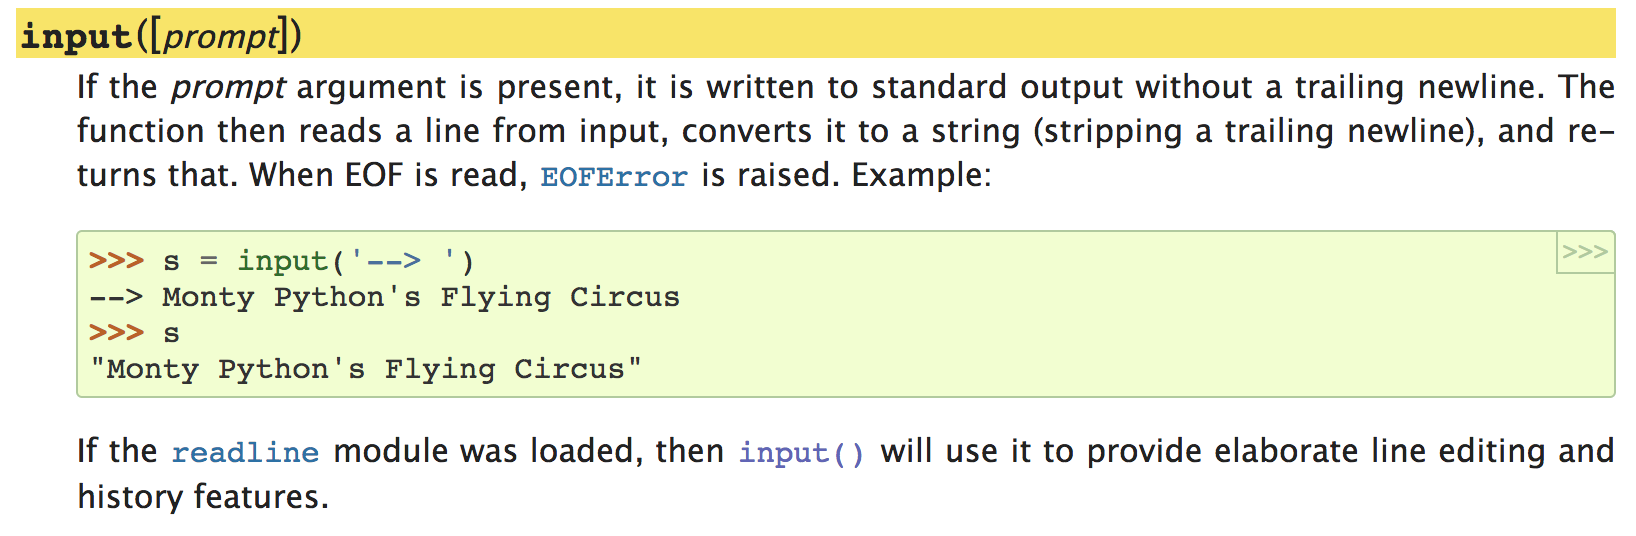
\includegraphics[width=.9\linewidth]{./python_docs.png}
\end{center}
\item So, let's analyze this, and try it
\end{itemize}
\subsection{How to Google well}
\label{sec:org114625d}
\begin{itemize}
\item Is it better to Google smaller questions or the entire problem?
\begin{itemize}
\item Why?
\end{itemize}
\item Where's the line between plagiarizing and utilizing the community?
\item What are some good websites for looking stuff up on?
\item Try:
\begin{itemize}
\item Stack overflow
\item Official Python Documentation
\end{itemize}
\end{itemize}
\section{Project 1}
\label{sec:org5eabebb}
A calculator

\begin{enumerate}
\item Ask the user to select an operation
\item Ask the user for the inputs of that operation
\item Perform the operation, print the result
\item Ask if the user wishes to use the calculator again
\begin{enumerate}
\item If yes, repeat
\item If no, exit
\end{enumerate}
\end{enumerate}

\section{Project 2}
\label{sec:org11628e9}
A game

\begin{enumerate}
\item Computer picks a random number between 1 and 100
\item Computer asks user for a guess
\item Computer tells user whether they are high, low, or correct
\item Give the user 10 guesses
\item When the users guesses it, tell them how many guesses it took
\item If the user doesn't get it in 10 guesses, print what the number was
\end{enumerate}

\subsection{Project 2 Extension}
\label{sec:orgf1eae7f}
\begin{itemize}
\item Can we teach the computer to intelligently make the best guess?
\item Switch the roles, have you pick the number, and the computer guess?
\item What's the maximum guesses it will take for the computer to get it in theory?
\end{itemize}
\end{document}
